\chapter{Introduzione}
\label{chap:introduzione}

\section{Convenzioni tipografiche}
Riguardo la stesura del testo, relativamente al documento sono state adottate le seguenti convenzioni tipografiche:
\begin{itemize}
	\item Gli acronimi, le abbreviazioni e i termini ambigui o di uso non comune menzionati vengono definiti nel glossario, situato alla fine del presente documento.
	\item Per la prima occorrenza dei termini riportati nel glossario viene utilizzata la seguente nomenclatura: \textit{parola}\glox.
	\item I termini in lingua straniera o facenti parti del gergo tecnico sono evidenziati con il carattere \textit{corsivo}.
\end{itemize}


\section{Organizzazione del testo}
Questa tesi è strutturata per fornire una visione dettagliata e comprensibile dell'esperienza di stage presso \myAzienda,
focalizzandosi sullo sviluppo di un'applicazione \gls{crplg}\glox e sullo studio di un ambiente di sviluppo in \gls{monorepog}\glox.
\\La suddivisione dei capitoli permette di seguire il percorso progettuale in modo chiaro e logico, dal contesto aziendale alle conclusioni finali. 
Di seguito è riportata l'organizzazione del testo:

\begin{description}
    \item[{\hyperref[chap:introduzione]{Introduzione:}}] Il capitolo introduttivo presenta una panoramica dell'azienda \myAzienda, il contesto dello stage, e fornisce una descrizione dettagliata dell'organizzazione della tesi.
    \item[{\hyperref[chap:stage_descrizione]{Descrizione dello stage:}}] In questo capitolo viene descritto il progetto di stage, inclusi gli obiettivi tecnici e professionali, le attività svolte, la pianificazione dettagliata e l'analisi preventiva dei rischi.
    \item[{\hyperref[chap:tecnologie_utilizzate]{Tecnologie utilizzate:}}] Questo capitolo elenca e descrive le tecnologie impiegate durante lo sviluppo dell'applicazione.
    \item[{\hyperref[chap:analisi_requisiti]{Analisi dei requisiti:}}] In questa sezione vengono descritti i casi d'uso, il monitoraggio dei requisiti e le tabelle che specificano le funzioni principali dell'applicazione.
    \item[{\hyperref[chap:design_coding]{Progettazione e codifica:}}] In questo capitolo verranno esaminati i \gls{designpatterng}\glox adottati, esemplificati con parti significative di codice, insieme a descrizioni dettagliate di alcune funzionalità chiave sviluppate.
    \item[{\hyperref[chap:studio_fattibilita]{Studio fattibilità app in \textit{monorepo}:}}] Questo capitolo esplora la fattibilità dello sviluppo dell'applicazione in un ambiente \gls{monorepog}\glox, descrivendo l'organizzazione iniziale, le problematiche rilevate, le soluzioni proposte e gli strumenti utilizzati per la gestione delle dipendenze.
    \item[{\hyperref[chap:conclusioni]{Conclusioni:}}] Il capitolo conclusivo presenta un consuntivo finale del lavoro svolto, una valutazione del raggiungimento degli obiettivi prefissati, le conoscenze acquisite durante lo stage, e una riflessione personale sull'esperienza complessiva.
    \item[{\hyperref[cap:bibliography]{Bibliografia e Sitografia:}}] Infine, vengono elencate le fonti bibliografiche e sitografiche consultate per la redazione della tesi.
\end{description}
\pagebreak
\section{L'azienda}

\myAzienda è un'azienda leader nel settore della produzione di forni professionali per la ristorazione, fondata nel 1990 e situata a Cadoneghe, in provincia di Padova, Italia.
\\Riconosciuta a livello internazionale per la qualità, l'affidabilità e l'innovazione dei suoi prodotti, UNOX è all'avanguardia nella tecnologia di cottura intelligente, che integra connettività avanzata e automazione.\footcite{site:unox_sito}

\subsection{Mission e Vision}
La \textit{mission} di \myAzienda è quella di contribuire al successo dei propri clienti offrendo soluzioni innovative e di alta qualità che migliorano le prestazioni e l'efficienza delle loro cucine.
L'azienda si impegna a fornire prodotti che combinano tecnologia avanzata e facilità d'uso, garantendo al contempo sostenibilità ambientale e risparmio energetico.
\\La \textit{vision} di UNOX si concentra sull'essere il punto di riferimento per l'innovazione nel settore della ristorazione professionale.
L'azienda punta a creare valore attraverso lo sviluppo continuo di tecnologie all'avanguardia e il miglioramento costante dei propri prodotti e servizi.

\subsection{Prodotti e Servizi}
UNOX offre una vasta gamma di forni professionali, noti per la loro efficienza, versatilità e innovazione tecnologica.
I prodotti principali includono:
\begin{itemize}
    \item Forni a convezione: Forni che utilizzano l'aria calda per cuocere il cibo in modo uniforme e veloce.
    \item Forni a vapore: Forni che utilizzano il vapore per cucinare in modo sano e preservare le proprietà nutrizionali degli alimenti.
    \item Sistemi di cottura intelligenti: Tecnologie integrate che permettono il controllo preciso dei processi di cottura e l'automazione delle operazioni.
    \item Forni combinati: Forni che combinano cottura a vapore e a convezione, ideali per una varietà di preparazioni culinarie.
\end{itemize}

\subsection{Connettività e Innovazione}
\myAzienda è pioniera nell'integrazione della connettività nei suoi prodotti, offrendo soluzioni che permettono il monitoraggio e il controllo remoto dei forni attraverso piattaforme digitali.
\\L'azienda ha sviluppato il progetto \gls{ddc}\glox, una piattaforma che utilizza i dati raccolti dai forni per ottimizzare i processi di cottura e fornire suggerimenti personalizzati agli chef.

\begin{figure}[H]
    \centering
    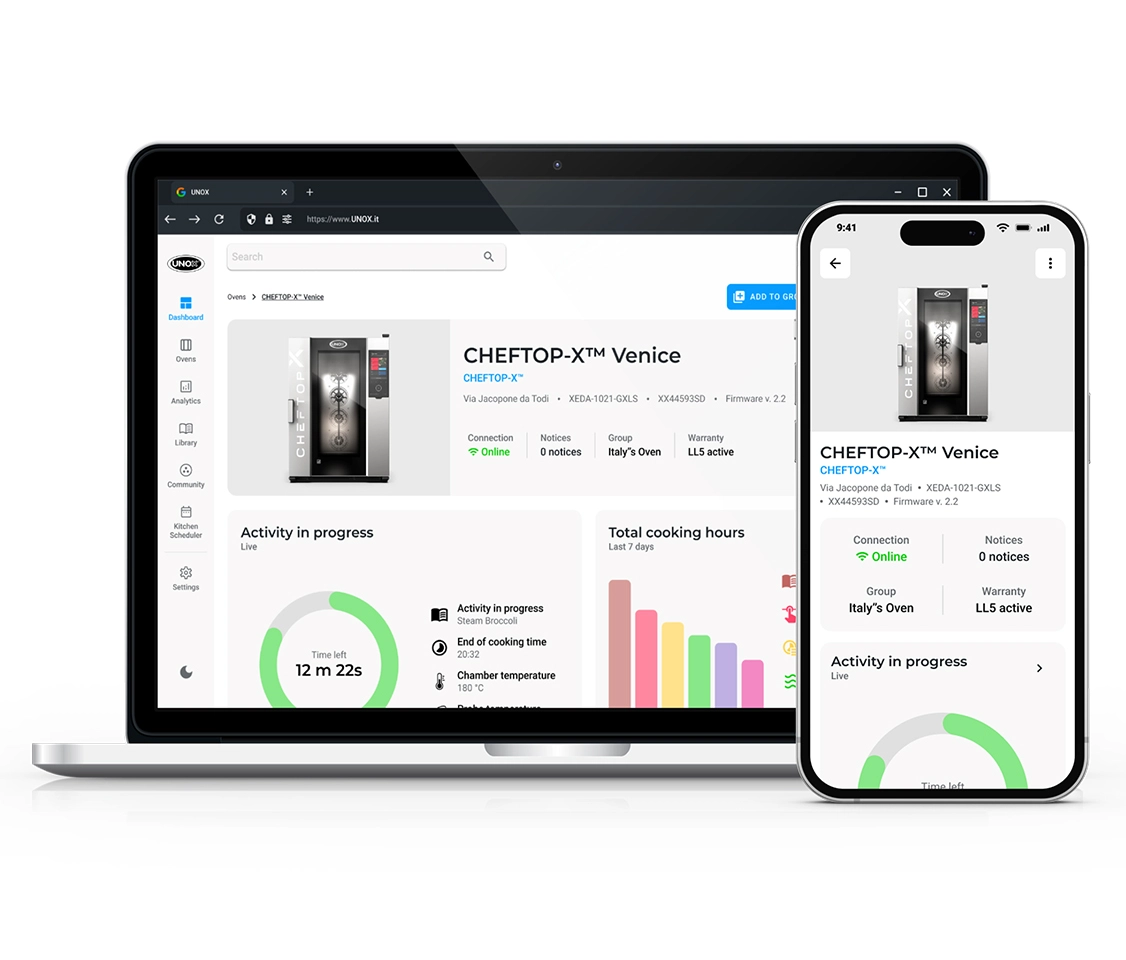
\includegraphics[alt={Immagine della applicazione \textit{DDC} su piattaforma \textit{Web e Mobile}}, height=10cm]{img/ddc.png}
    \caption{App \textit{DDC}: Applicazione \textit{DDC} su piattaforma \textit{Web} e Mobile}
    \label{fig:ddc}
\end{figure}


\section{Lo stage}
L'offerta di stage mi ha immediatamente intrigato per il suo focus su un progetto specifico vitale per l'azienda, piuttosto che un semplice esercizio accademico.
Questo aspetto ha richiesto un impegno significativo e una collaborazione intensa con diversi \textit{team} per portare a termine un progetto cruciale per l'azienda.
Nel contesto aziendale esistono due app chiamate \gls{ddc}\glox e \gls{ddcserviceg}\glox.
\begin{itemize}
    \item \textit{DDC} ha come utilizzatori i proprietari dei forni che utilizzano questa app per le funzionalità connesse dei loro dispositivi.
    \item \textit{DDC Service} ha come utilizzatori personale tecnico, personale responsabile di manutenzione dei forni e utenti addetti al \textit{Service}.
\end{itemize}
Per rispondere alle esigenze aziendali, è stato necessario avviare lo sviluppo di una nuova app \textit{DDC Service} con una prospettiva moderna e che sia multi-piattaforma.
Durante il mio stage presso \myAzienda, ho lavorato principalmente sull'avvio dello sviluppo di questa app, il mio obiettivo principale è stato ristrutturare e sviluppare completamente da zero \textit{DDC Service} precedentemente limitata alla piattaforma \textit{Web}.
Ho esteso le funzionalità di \textit{DDC Service} per renderla compatibile con dispositivi \textit{Android, iOS e Web}, integrando questa nuova versione nell'esistente \gls{monorepog}\glox di \textit{DDC}.
\\Questo approccio ha permesso di condividere il \gls{designsystemg}\glox e sfruttare l'infrastruttura esistente per ottimizzare l'efficienza e la manutenibilità del codice.
\\Durante il periodo di stage, ho collaborato attivamente con il \textit{team} di sviluppo, design e progettazione per implementare le prime funzionalità richieste per l'applicazione, rispettando le linee guida e assicurando la compatibilità su tutte le piattaforme \textit{target}.
Questa esperienza mi ha fornito competenze pratiche nello sviluppo software multi-piattaforma e una comprensione approfondita della progettazione scalabile e della gestione delle risorse tecniche in un ambiente \textit{monorepo}.


\newpage